\section{Datenmigration von MySQL zu CouchDB}
\label{datenmigration}

In diesem Kapitel soll auf technischer Ebene die Migration von bestehenden Daten aus einer MySQL-Datenbank in eine Couch-Datenbank erl�utert werden. Zur besseren Veranschaulichung wird auch dies an einem Beispiel gezeigt.  

\begin{figure}
	\centering
		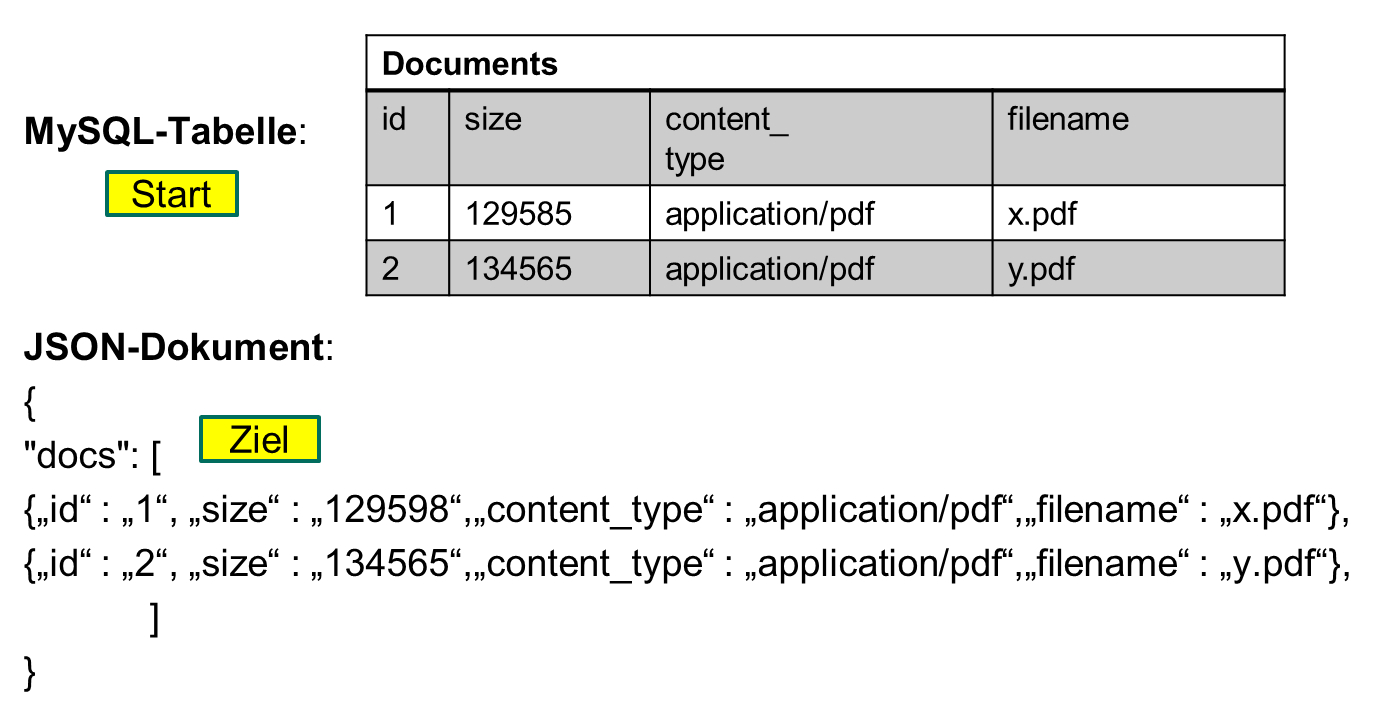
\includegraphics[width=1.00\textwidth]{figures/beispielDatenmigration.png}
	\caption{Gleiche Daten gespeichert in einer MySQL-Tabelle und in einem CouchDB-Dokument.}
	\label{fig:beispielDatenmigration}
\end{figure}

Abbildung \ref{fig:beispielDatenmigration} zeigt eine MySQL-Tabelle mit zwei Datens�tzen (Zeilen), die in das darunterliegende JSON-Dokument �berf�hrt werden m�ssen, um von CouchDB interpretiert werden zu k�nnen. Das Dokument enth�lt ein Array (\textit{docs}), welches f�r jede Zeile einen Eintrag enth�lt. Ziel ist es nun, die Daten aus der MySQL-Tabelle in JSON-Format zu �berf�hren. Der hier beschriebene Vorgang unterliegt der Annahme, dass die Daten ohne Transformationsschritt, wie beispielsweise eine Zusammenf�hrung zweier Datenbanken, durchgef�hrt werden kann. F�r die reine �bertragung kann eine SQL-Anfrage benutzt werden, die die Daten Attribut f�r Attribut aus der Datenbank ausliest, konkateniert und zeilenweise in ein Dokument schreibt. Abbildung \ref{fig:SQL-Befehl} zeigt diese Anfrage. Im Beispiel werden die Daten der Tabelle \textit{documents} aus der Datenbank \textit{olio} ausgelesen und in die Datei \textit{documents.json} geschrieben. Bei der Wahl des Speicherortes f�r das Dokument ist darauf zu achten, dass MySQL entsprechende Zugriffsrechte auf dieses Verzeichnis hat. 

\begin{figure}
	\centering
		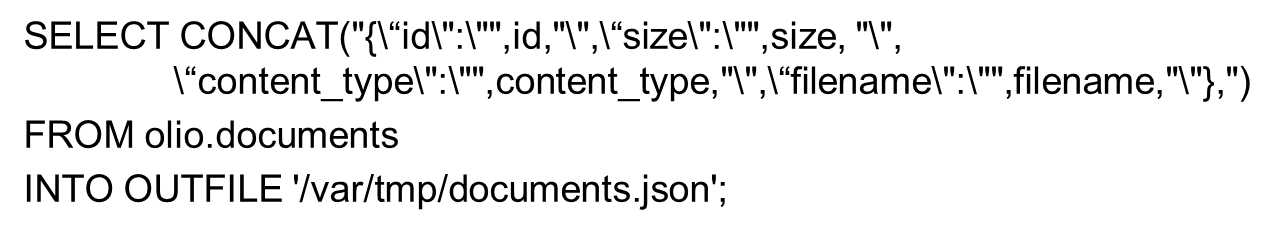
\includegraphics[width=0.90\textwidth]{figures/SQL-Befehl.png}
	\caption{SQL-Anfrage zum Auslesen der Tabelle \textit{documents} in der Datenbank \textit{olio}.}
	\label{fig:SQL-Befehl}
\end{figure}

Das durch die SQL-Abfrage entstehende Dokument ist allerdings noch nicht in der gew�nschten Form, da bisher nur die Daten untereinander geschrieben wurden. Es fehlen noch die geschwungenen Klammern, die das gesamte Dokument eingrenzen, und das Array, um die Datens�tze zusammenzufassen. Dies kann beispielsweise �ber ein Ruby-Skript gel�st werden, welches die entsprechenden Zeichen in das Dokument (hier: \textit{documents.json}) einf�gt.\\
Bis zu diesem Schritt wei� CouchDB allerdings noch nichts von der Existenz der Daten. Zwar liegen diese zusammengefasst in einem Array vor, jedoch m�ssen diese nun noch in CouchDB geladen werden. Hierf�r h�lt CouchDB die \textit{Bulk-Load}-Funktion bereit. Mit dieser Funktion k�nnen viele Datens�tze auf einmal in CouchDB geladen werden. Gegen�ber der Einzelabspeicherung von Daten kann durch diese Funkion viel Zeit gewonnen werden, wenn die Datens�tze entsprechend gro� sind. 

\begin{figure}
	\centering
		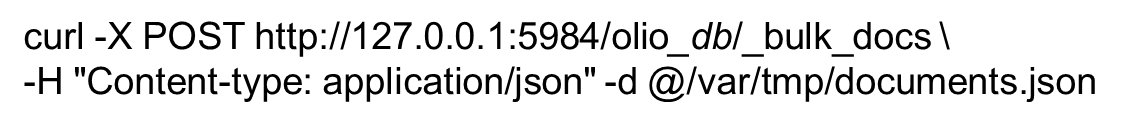
\includegraphics[width=0.90\textwidth]{figures/curlBefehl.png}
	\caption{Curl-Befehl zum gleichzeitigen Laden mehrerer Datens�tze in CouchDB mit \textit{Bulk Load}.}
	\label{fig:curlBefehl}
\end{figure}

Abbildung \ref{fig:curlBefehl} zeigt den Befehl zum gleichzeitigen Laden vieler Daten. Da CouchDB eine REST-Schnittstelle anbietet, wird hierzu das Kommandozeilenwerkzeug \textit{Curl} verwendet, das entwickelt wurde, um Daten mit Url-Syntax unter anderem mittels HTTP, SSH oder FTP zu �bertragen \cite{curl}.\\
Der Zugriff auf die Datenbank erfolgt �ber eine einfache Url (hier Localhost auf dem gleichen Rechner �ber Port 5984), an die der Name der Datenbank (\textit{olio\_db}) angehangen wird. Auch der auszuf�hrende Befehl \textit{\_bulk\_docs} ist Teil der Url. Die Datei, in der die zu ladenden Daten liegen, wird �ber die Option \textit{-d} angegeben. Zus�tzlich muss noch der Typ der �bertragenen Daten angegeben werden, in diesem Falll JSON.\\
CouchDB geht bei einem Bulk Load so vor, dass es f�r jeden Eintrag im Array ein eigenes Dokument in der entsprechenden Datenbank anlegt. Der Nachteil dieses Verfahrens ist allerdings, dass bei vielen Attributen in einer Datenbank der SQL-Befehl entsprechend lang wird. Eine M�glichtkeit der Vereinfachung ist, beispielsweise ein Ruby-Skript zu erstellen, dem als Parameter der Datenbankname, der Tabellenname und die entsprechenden Attribute �bergeben werden und welches die Anfrage automatisch erstellt. Durch die Parametrisierung wird eine ausreichende Flexibilit�t erreicht, um die Daten aus verschiedenen Datenbanken in CouchDB zu laden, ohne lange Befehle von Hand schreiben zu m�ssen.